% Options for packages loaded elsewhere
\PassOptionsToPackage{unicode}{hyperref}
\PassOptionsToPackage{hyphens}{url}
%
\documentclass[
]{article}
\usepackage{lmodern}
\usepackage{amssymb,amsmath}
\usepackage{ifxetex,ifluatex}
\ifnum 0\ifxetex 1\fi\ifluatex 1\fi=0 % if pdftex
  \usepackage[T1]{fontenc}
  \usepackage[utf8]{inputenc}
  \usepackage{textcomp} % provide euro and other symbols
\else % if luatex or xetex
  \usepackage{unicode-math}
  \defaultfontfeatures{Scale=MatchLowercase}
  \defaultfontfeatures[\rmfamily]{Ligatures=TeX,Scale=1}
\fi
% Use upquote if available, for straight quotes in verbatim environments
\IfFileExists{upquote.sty}{\usepackage{upquote}}{}
\IfFileExists{microtype.sty}{% use microtype if available
  \usepackage[]{microtype}
  \UseMicrotypeSet[protrusion]{basicmath} % disable protrusion for tt fonts
}{}
\makeatletter
\@ifundefined{KOMAClassName}{% if non-KOMA class
  \IfFileExists{parskip.sty}{%
    \usepackage{parskip}
  }{% else
    \setlength{\parindent}{0pt}
    \setlength{\parskip}{6pt plus 2pt minus 1pt}}
}{% if KOMA class
  \KOMAoptions{parskip=half}}
\makeatother
\usepackage{xcolor}
\IfFileExists{xurl.sty}{\usepackage{xurl}}{} % add URL line breaks if available
\IfFileExists{bookmark.sty}{\usepackage{bookmark}}{\usepackage{hyperref}}
\hypersetup{
  hidelinks,
  pdfcreator={LaTeX via pandoc}}
\urlstyle{same} % disable monospaced font for URLs
\usepackage{graphicx}
\makeatletter
\def\maxwidth{\ifdim\Gin@nat@width>\linewidth\linewidth\else\Gin@nat@width\fi}
\def\maxheight{\ifdim\Gin@nat@height>\textheight\textheight\else\Gin@nat@height\fi}
\makeatother
% Scale images if necessary, so that they will not overflow the page
% margins by default, and it is still possible to overwrite the defaults
% using explicit options in \includegraphics[width, height, ...]{}
\setkeys{Gin}{width=\maxwidth,height=\maxheight,keepaspectratio}
% Set default figure placement to htbp
\makeatletter
\def\fps@figure{htbp}
\makeatother
\setlength{\emergencystretch}{3em} % prevent overfull lines
\providecommand{\tightlist}{%
  \setlength{\itemsep}{0pt}\setlength{\parskip}{0pt}}
\setcounter{secnumdepth}{-\maxdimen} % remove section numbering
\usepackage{color}
\usepackage{soulutf8}
\usepackage{color}
\usepackage{soulutf8}
\usepackage{color}
\usepackage{soulutf8}
\usepackage{color}
\usepackage{soulutf8}
\usepackage{color}
\usepackage{soulutf8}
\usepackage{color}
\usepackage{soulutf8}
\usepackage{color}
\usepackage{soulutf8}
\usepackage{color}
\usepackage{soulutf8}
\usepackage{color}
\usepackage{soulutf8}
\usepackage{color}
\usepackage{soulutf8}

\author{}
\date{}

\begin{document}

\hypertarget{header-n2}{%
\subsection{Meeting Notes}\label{header-n2}}

\hypertarget{header-n3}{%
\subsection{Looked at Since Last Meeting}\label{header-n3}}

\begin{itemize}
\item
  \textbf{Big Update to Linkage Renderer}

  The linkage rendering has been accomplished, and it has grown in scope
  fairly substantially. Namely, the broken 4-gon from before now renders
  nicely going from this:

  \begin{figure}
  \centering
  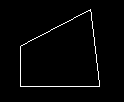
\includegraphics{C:/Users/evan/Documents/configuration-spaces/images/image-20200213111607569.png}
  \caption{}
  \end{figure}

  To this; fixed, with points highlighted and antialiasing enabled:

  \begin{figure}
  \centering
  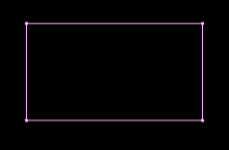
\includegraphics{C:/Users/evan/Documents/configuration-spaces/images/image-20200224150420545.png}
  \caption{}
  \end{figure}

  Obviously this is now functional, but I also have added a 'show
  alternate switch option' so we can see this:

  \begin{figure}
  \centering
  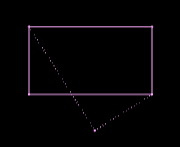
\includegraphics{C:/Users/evan/Documents/configuration-spaces/images/image-20200224150600536.png}
  \caption{}
  \end{figure}

  And also the coordinates and lengths can be edited with this user
  interface:

  \begin{figure}
  \centering
  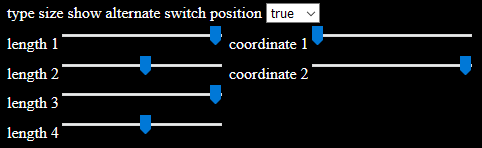
\includegraphics{C:/Users/evan/Documents/configuration-spaces/images/image-20200224150806060.png}
  \caption{}
  \end{figure}

  This is all good, but the problem is that the lengths and coordinates
  can be altered to provide configurations that don't fulfill this
  equation: \(\sum_{k=i}^j \boldsymbol\alpha_k \ell_k = 0 \) that
  ensures that the polygon connects at the end.
\item
  \textbf{Thinking of Range Limiting and it's Topological Consequences}

  Leading on from the last point, I believe it is possible to calculate
  analytically (geometrically) the range of each linkage, and using a
  conjecture from Kevin Walker about how the order of linkages (need to
  check this) doesn't matter, essentially as addition in \(\mathbb R^2\)
  is commutative.
\end{itemize}

\hypertarget{header-n19}{%
\subsection{Current Problems}\label{header-n19}}

\begin{itemize}
\item
  Describing linkages for orientable 2-manifolds.
\item
  Work through the ideas behind the 'range limiting' of the linkage
  renderer. Could this lead to a way to iterate different manifolds?
\end{itemize}

\hypertarget{header-n25}{%
\subsection{Current Tasks}\label{header-n25}}

\begin{itemize}
\item
  Add range limiters to the coordinate selector in the linkage renderer
  so the linkage can't be put into unattainable positions.
\item
  Fix the dynamic size choice in the linkage renderer
\item
  Add angle helper class to the linkage renderer
\end{itemize}

\hypertarget{header-n33}{%
\subsection{Links}\label{header-n33}}

Kapovich and Millson \\
https://arxiv.org/pdf/math/9803150.pdf

Robert Ghrist\\
https://www.math.upenn.edu/\textasciitilde ghrist/EAT/EATchapter1.pdf

Gaiane Panina\\
http://amj.math.stonybrook.edu/pdf-Springer-final/017-0070.pdf

Kevin Walker\\
https://canyon23.net/math/1985thesis.pdf

"On the Conjecture of Kevin Walker" \hl{unread}\\
https://arxiv.org/pdf/0708.2995.pdf

Some Lecture Notes from a Course on this, talks about chambers in a way
that sounds good \hl{unread} \\
http://homepages.warwick.ac.uk/\textasciitilde maskas/courses/schuetz1.pdf

\hypertarget{header-n40}{%
\subsection{Project Notes}\label{header-n40}}

\hypertarget{header-n41}{%
\subparagraph{\texorpdfstring{Thinking about the Fundamental Group, Free
Products and the \((C_4, (a,b,a,b))\)
}{Thinking about the Fundamental Group, Free Products and the (C\_4, (a,b,a,b)) }}\label{header-n41}}

Looking at this manifold:

\begin{figure}
\centering
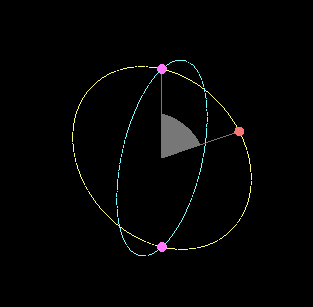
\includegraphics{C:/Users/evan/Documents/configuration-spaces/images/image-20200211170146292.png}
\caption{}
\end{figure}

We can find a homotopy between this and the \(\bigwedge_3 \mathbb S^1\)
as follows: \hl{somehow I think I might want to redraw this}

\begin{figure}
\centering
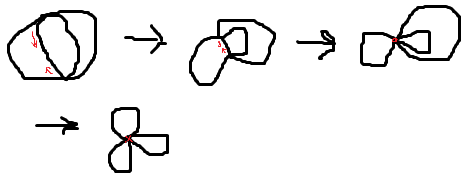
\includegraphics{C:/Users/evan/Documents/configuration-spaces/images/image-20200225121214537.png}
\caption{}
\end{figure}

This then means we can apply the Siefert-van Kampen Theorem and get that
\(\Pi_1(M((C_4, (a,b,a,b)))) \simeq \bold *_3 \mathbb Z\).

This is interesting if we remember the meaning of the configuration
space and the fundamental group.

We first have to follow our fixed point of intersection (red in the
diagram above) and work out what that means in our linkage. This is a
position where the switch has only one state. \hl{I think} without loss
of generality, depending on how we manipulate our manifold, this will be
the position where the coordinate of the first linkage is either
\(\frac \pi 2\) or \(\frac {3\pi} 2\) and the structure follows a
straight line.

Given the free product and the fundamental group, this leads to an idea
of a 'loop' in our linkage where we end up back at this fixed point, and
the fact it's an \(\bigwedge_3 \mathbb S^1\) implies that there is 3
unique ways of 'looping' back to this position.

To outline a potential form these three loops might take:

\hl{non complete}

\hypertarget{header-n52}{%
\subparagraph{\texorpdfstring{Describing the Homotopy between the 1-arm,
2-arm and n-arm and the \(\mathbb T^n \)\hl{work in
progress}\_}{Describing the Homotopy between the 1-arm, 2-arm and n-arm and the \textbackslash mathbb T\^{}n work in progress\_}}\label{header-n52}}

\hypertarget{header-n53}{%
\subparagraph{\texorpdfstring{\emph{Describing the Homotopy between a
\$(C}4, (a,b,a,b))\( and the Intersecting \)\textbackslash mathbb
S\^{}1\$'s\_}{Describing the Homotopy between a \$(C4, (a,b,a,b)) and the Intersecting \textbackslash mathbb S\^{}1\$'s\_}}\label{header-n53}}

I believe this holds for all \((C_4, (a,b,a,b))\) with
\(a,b \in \mathbb R^+\) and \(a \not = b\).

This provides an interesting configuration space
\(M((C_4, (a,b,a,b)))\), which we'll shorten to \(M\) for this exercise,
that is composed of a two \(\mathbb S^1\)'s which are disjoint besides
two points (call this manifold \(X\) for now). This looks like so:

\begin{figure}
\centering
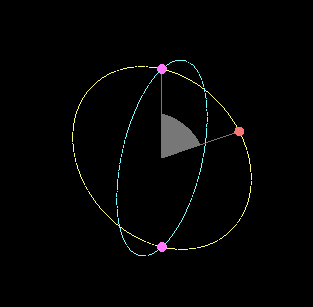
\includegraphics{C:/Users/evan/Documents/configuration-spaces/images/image-20200211170146292.png}
\caption{}
\end{figure}

To prove this we have to find a pair of maps:

\[f: M \rarr X \\
g: X \rarr M \\
s.t. f \, \circ g \simeq Id_X \, and \, g \, \circ f \simeq Id_{M}\]

This is not too hard, using the definition of the Moduli Space that I
have outlined, we can see that any position of the manifold can be
indexed with two values, as we have 2 degrees of freedom.

The first value is the angle subtended between \(\hat e _y\) and the
direction of the link connected to the base on the left. \hl{add a
diagram here using \texttt{Polygon} with angle helpers}

The second value can be expressed with a Boolean, as we have a switch
formed with the remaining two links, however, the two possible values
are equivalent if the first value is \(\frac \pi 2\) or
\(\frac {3 \pi} 2\). This happens because the first two links line up
(\hl{add diagram}) meaning that the angle between the 3rd and 4th link
is either 0 or \(\pi\) meaning that flipping it doesn't produce a new
state.

Hence:

\begin{enumerate}
\def\labelenumi{\arabic{enumi}.}
\item
  Any point \((a_1,a_2)\) in \(M((C_4, (2,1,2,1)))\) is also in
  \(\mathbb S^1 \times \mathbb S^0\) but fixing \((0,1) = (0,0)\) and
  \((\pi,0) = (\pi, 1)\).
\item
  Any point \(\boldsymbol{x}\) in \(X\) is on one of the
  \(\mathbb{S^1}\)'s that \(X\) is composed of, at an angle we'll call
  \(\theta\).
\end{enumerate}

Without loss of generality, as the manifold is the same if you rotate it
\(\frac \pi 2\) about the \(y\)-axis, we can specify the
\(\mathbb S^1\)'s that make up \(X\) and call them \(B\) and \(Y\) (blue
and yellow matching the diagram).

Then define:

\[f: M \rarr X \\
f := f((a_1,a_2)) =
\begin{cases}
\theta = a_1 \text{ around } Y \text{ if } a_2 = 0
\\
\theta = a_1 \text{ around } B \text{ if } a_2 = 1
\\
\theta = a_1 \text{ in } B \cap Y  \text{ if } a_1 = 0 \text{ or } a_1 = \pi \\
\end{cases}\]

and:

\[\\
g: X \rarr M \\
g := g(\boldsymbol{x}) = (a_1, a_2)  \\
\text{where } a_1 \text{ is } \theta \text{ and }  a_2 = 
\begin{cases}
0 \text{ if } \boldsymbol x \in Y
\\
1 \text{ if } \boldsymbol x \in B/Y
\end{cases}\]

Now evaluating:

\[(g \circ f)((a_1,a_2)) = g \left( \boldsymbol x := \begin{cases}
\theta = a_1 \text{ around } Y \text{ if } a_2 = 0
\\

\theta = a_1 \text{ around } B \text{ if } a_2 = 1\\
\theta = a_1 \text{ in } B \cap Y  \text{ if } a_1 = 0 \text{ or } a_1 = \pi \\
\end{cases} \right) 

= 

\left( \theta, 
\begin{cases}
0 \text{ if } \boldsymbol x \in Y
\\
1 \text{ if } \boldsymbol x \in B
\end{cases}
\right)

= (a_1, a_2)

\\

=> g \, \circ f \simeq Id_{M}\]

and:

\[(f \circ g)(\boldsymbol x) = f \left( \left(\theta, 
\begin{cases}
0 \text{ if } \boldsymbol x \in Y
\\
1 \text{ if } \boldsymbol x \in B/Y
\end{cases} \right) \right)
=
\boldsymbol x
\\
=> f \circ g \simeq Id_X\]

Proving that \(M \simeq X\).

\hypertarget{header-n78}{%
\subparagraph{\texorpdfstring{\emph{Describing the homotopy between the
switch and \(\mathbb S^0 \) \hl{work in
progress}}}{Describing the homotopy between the switch and \textbackslash mathbb S\^{}0  work in progress}}\label{header-n78}}

\hypertarget{header-n79}{%
\subparagraph{\texorpdfstring{\emph{Definition and Intuition of Nash
Isomorphisms}
}{Definition and Intuition of Nash Isomorphisms }}\label{header-n79}}

A Nash function \(f\) on a set \(U\) satisfies there exists a polynomial
\(P\) in \(x\) and \(f(x)\) such that
\(\forall x \in U, \,\,\,\, P(x,f(x)) = 0\)

A Nash Manifold is an example of a \(U\) from the above definition that
also has the structure of a manifold.

From Wikipedia, this result looks like it could be helpful:

\begin{quote}
"More generally, a smooth manifold admits a Nash manifold structure if
and only if it is diffeomorphic to the interior of some compact smooth
manifold possibly with boundary."

https://en.wikipedia.org/wiki/Nash\_functions
\end{quote}

\hypertarget{header-n86}{%
\subparagraph{\texorpdfstring{\emph{Working with the 5-Cycle Linkage to
get 2-Manifolds} \hl{work in
progress}}{Working with the 5-Cycle Linkage to get 2-Manifolds work in progress}}\label{header-n86}}

\hypertarget{header-n87}{%
\subparagraph{\texorpdfstring{\emph{The Classification Theorem for
2-Manifolds}}{The Classification Theorem for 2-Manifolds}}\label{header-n87}}

We can describe all 2-manifolds with a genus and an orientability.
Probably write more and some drawings here if relevant, delete in a
couple weeks if not going to be used.

\hypertarget{header-n89}{%
\subparagraph{\texorpdfstring{\emph{Current Working Definition of a
Linkage, Configuration Space and the State of a
Linkage}}{Current Working Definition of a Linkage, Configuration Space and the State of a Linkage}}\label{header-n89}}

A linkage is composed of a SCaF graph \(L\) paired with a length
function on the edges (\(\ell\) ).

A configuration or moduli space \(C((L,\ell))\) is defined like so:\\
\( M(L,\ell) := \{(\boldsymbol\alpha_1,..., \boldsymbol\alpha_n) \in (\mathbb S^1)^n | for \, any \, cycle \, l_i, ..., l_j\, in \, L: \sum_{k=i}^j \boldsymbol\alpha_k \ell_k = 0 \}\)\\
modulo distance preserving isometries of the plane.

When we work with a linkage we need a way to consistently talk about the
position that the links are in. The way I will work with this is to
consider the fixed link to be oriented in the x-axis and then measure
the angle that each link makes to the y-axis clockwise, working with the
links in chain from the left of the base.

For now I am going to ignore forks, as they would require some more
complex thought to decide how to work with their state.

If this is a polygon we will end up working round to the other side of
the base link. Note that; unless the 3rd to last link ends up in the
same position as the right of the base, we will be able to index the
last two links using a single Boolean value as it will form a switch
(two fixed points with two links between them).

If this is not a polygon then we have either an n-arm or nothing
connected to both sides of the base link, and we can define these
working with the left one, followed by the right one looking at the
angles and working up through each arm in turn.

\hypertarget{header-n96}{%
\subparagraph{\texorpdfstring{\emph{Examples of Manifolds and the
Linkages that Display them as Configuration
Spaces}}{Examples of Manifolds and the Linkages that Display them as Configuration Spaces}}\label{header-n96}}

\(\mathbb S^1 \): A manifold that leads to a \(\mathbb S^1\)
configuration space is easy to find, as it is the configuration space of
a single linkage at the origin.

\(\mathbb S^2\)?

\(\mathbb S^1 \bigcup \, \mathbb S^1 = T^2\): A manifold with the
configuration space two disjoint spheres is also pretty okay. This is
the linkage represented by a pair of rigid links connected by a linkage
that pivots freely around any angle.

\hypertarget{header-n100}{%
\subparagraph{\texorpdfstring{\emph{What Happens to the Configuration
Space as one modifies the Linkage}
}{What Happens to the Configuration Space as one modifies the Linkage }}\label{header-n100}}

"Adding to the Chain"

When we add another link onto the end of a simple chain of length \(n\)
we go from a configuration space of \(\bigcup_1^n \, \mathbb S^1 = T^n\)
to one of \(\bigcup_1^{n+1} \, \mathbb S^1 = T^{n+1}\), in fact, it
seems that if we add another link to a system with a configuration space
\(M\) we will get a configuration space of \(M \bigcup \mathbb \, S^1\).
(prove this?)

\hypertarget{header-n103}{%
\subparagraph{\texorpdfstring{\emph{Is any Manifold Diffeomorphic to the
Configuration Space of a well defined
Linkage?}}{Is any Manifold Diffeomorphic to the Configuration Space of a well defined Linkage?}}\label{header-n103}}

Robert Ghrist states on page 12 of his book \emph{Elementary Applied
Topology} that:
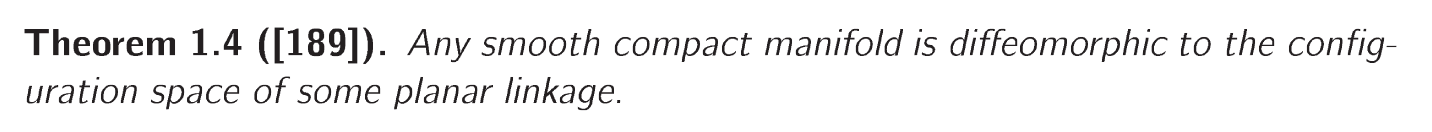
\includegraphics{C:/Users/evan/Documents/configuration-spaces/images/image-2020020252237727 pm.png}

https://www.math.upenn.edu/\textasciitilde ghrist/EAT/EATchapter1.pdf

However, Kapovich and Millson disagree with this in their paper below:

\begin{figure}
\centering
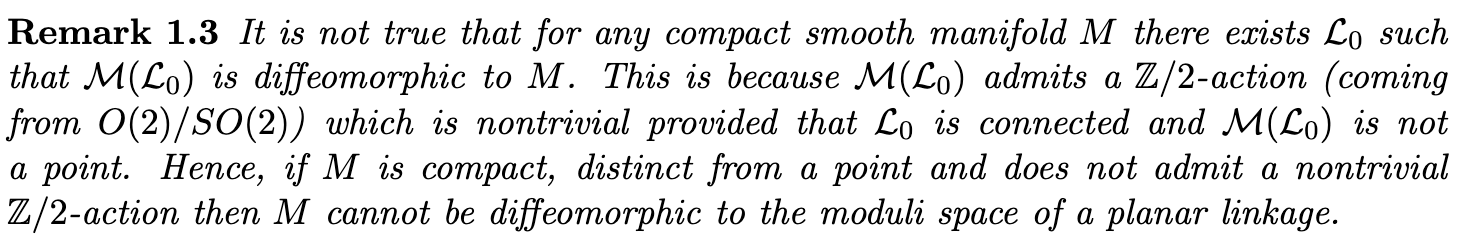
\includegraphics{C:/Users/evan/Documents/configuration-spaces/images/image-2020020252749698 pm.png}
\caption{}
\end{figure}

https://arxiv.org/pdf/math/9803150.pdf

At first glace I believe this is essentially telling us that not every
manifold can be expressed as the configuration of some linkage as these
configuration spaces can be transformed in some way (corresponding to
moving the linkage in the plane in which it resides, like flipping it
perhaps) and thus for any manifold that can't admit this transformation,
it can't be diffeomorphic to a configuration space.

I think the best way to work out what is going on here is to work with
the definitions of configuration space of a linkage, and decide if this
relates to the differing theorem. It seems unlikely that Ghrist is
stating his theorem more strongly without reason, given the cited source
is Kapovich and Millson's paper.

\hypertarget{header-n111}{%
\subparagraph{\texorpdfstring{\emph{Robert Ghrist Defines a
Configuration
Space:}}{Robert Ghrist Defines a Configuration Space:}}\label{header-n111}}

Robert Ghrist defines a configuration space as follows (also page 12 of
his book):

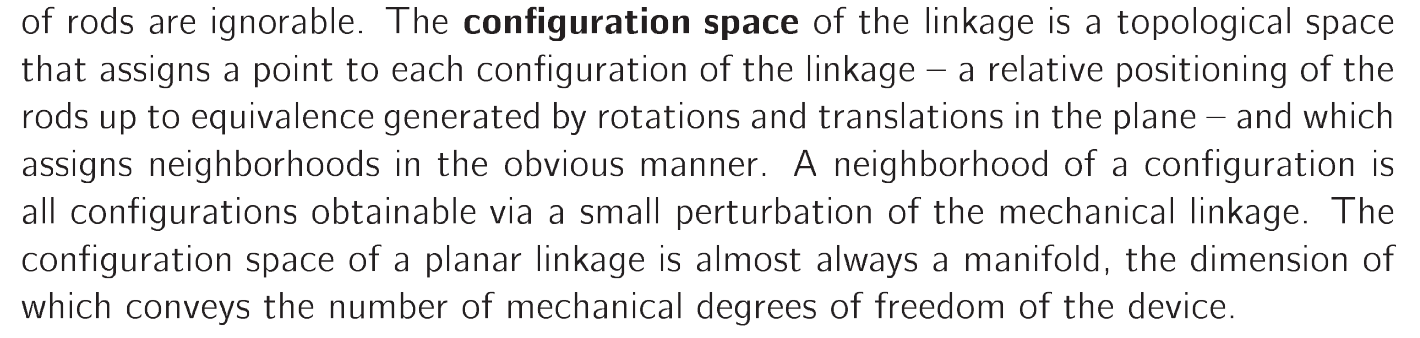
\includegraphics{C:/Users/evan/Documents/configuration-spaces/images/image-2020020254030088 pm.png}

https://www.math.upenn.edu/\textasciitilde ghrist/EAT/EATchapter1.pdf

This has some points to take away, namely we \textbf{are} assigning a
distinct point to each layout of the linkage, but we \textbf{are not}
considering rotations and reflections of the plane as different
configurations.

Also, the point \emph{'almost always a manifold'} should also be
addressed, this can be narrowed down by assuming that the linkages we
look at can never fit into a straight line; this can be found here
http://amj.math.stonybrook.edu/pdf-Springer-final/017-0070.pdf in Gaiane
Panina's paper, but should probably trace the reference to find it's
original source, likely Kapovich and Millson.

\hypertarget{header-n117}{%
\subparagraph{\texorpdfstring{\emph{Kapovich and Millson Define a Moduli
Space}}{Kapovich and Millson Define a Moduli Space}}\label{header-n117}}

Firstly, we should address the difference in terminology used by the
authors here, it seems that in this context, looking at linkages the
Moduli Space and the Configuration Space are the same thing.

This is strongly suggested in this paper by Gaiane Panina on the Moduli
Space of Planar Linkages here:

\begin{figure}
\centering
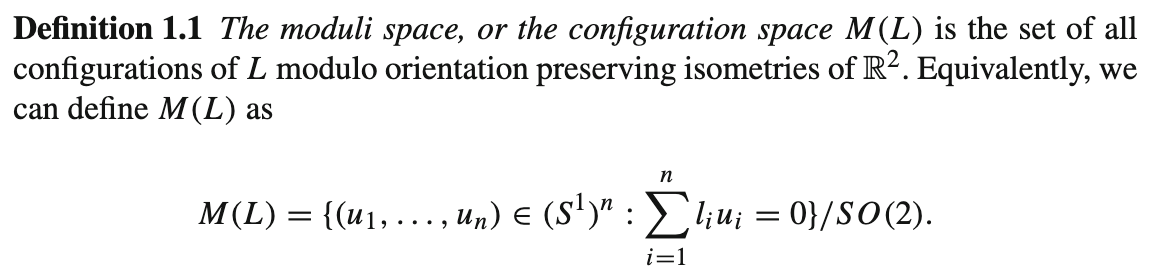
\includegraphics{C:/Users/evan/Documents/configuration-spaces/images/image-2020020255856993 pm.png}
\caption{}
\end{figure}

http://amj.math.stonybrook.edu/pdf-Springer-final/017-0070.pdf

However, Kapovich and Millson definitely make a point about the

\end{document}
